\documentclass[12pt,a4paper,oneside]{report}

\usepackage[utf8]{inputenc}
\usepackage[T1]{fontenc}
\usepackage[spanish,es-tabla]{babel}
\usepackage{amsmath,amssymb}
\usepackage{booktabs}
\usepackage{csquotes}
\usepackage{enumitem}
\usepackage{float}
\usepackage{geometry}
\usepackage{graphicx}
\usepackage{hyperref}
\usepackage{listings}
\usepackage{siunitx}
\usepackage{xcolor}

\geometry{margin=2.7cm}
\graphicspath{{../experiments/results/}{assets/}}
\hypersetup{
  colorlinks=true,
  linkcolor=black,
  citecolor=black,
  urlcolor=blue
}
\sisetup{
  output-decimal-marker={,},
  per-mode=symbol,
  detect-all=true
}
\setlist{itemsep=0.2em, topsep=0.4em}
\lstset{
  basicstyle=\ttfamily\small,
  breaklines=true,
  columns=fullflexible,
  frame=single,
  rulecolor=\color{black!25},
  numbers=left,
  numberstyle=\tiny\color{black!50},
  xleftmargin=1.5em,
  framexleftmargin=1.2em
}

\title{
  \textbf{Diseño y evaluación por simulación de un banco de pruebas de QKD BB84 en time-bin con estados señuelo}\\[0.5em]
  \large Proyecto Final Integrador -- Ingeniería en Telecomunicaciones
}
\author{Universidad Nacional de San Martín}
\date{2026}

\begin{document}

\maketitle

\chapter*{Resumen}
\phantomsection
\addcontentsline{toc}{chapter}{Resumen}

Este trabajo presenta el diseño y la evaluación por simulación de un banco de pruebas de distribución cuántica de claves basado en BB84 con codificación \textit{time-bin} para un enlace de dos nodos. El objetivo es estudiar qué información confiable puede obtenerse antes de construir el banco físico y qué resultados exigen revisar el modelo. Se analizan la tasa de error cuántico de bit (QBER), la tasa tamizada, un indicador ideal de posprocesamiento y estimadores asintóticos con y sin estados señuelo. El indicador ideal no se interpreta como tasa secreta para una fuente coherente débil.

La metodología usa SeQUeNCe 0.8.5 con una corrección local documentada para el error de fase del interferómetro. Se construye un escenario Alice--Bob con canal cuántico, canales clásicos, fuente coherente débil y receptor \textit{time-bin}. Se ejecutan cuatro barridos: distancia, eficiencia y conteos oscuros, visibilidad, y comparación con y sin estados señuelo. Cada punto reúne \PThreeRepetitions{} repeticiones deterministas; QBER se informa con intervalo de Wilson y las tasas con intervalo t del 95\%. La corrida exporta datos agregados y por repetición, semillas, conteos, metadatos y hashes.

El control de consistencia entre tasa simulada y referencia analítica cambia de régimen entre \num[round-mode=places,round-precision=2]{\PThreeTransitionLowKm} y \SI[round-mode=places,round-precision=2]{\PThreeTransitionHighKm}{\kilo\meter}; esta transición diagnostica temporización y contabilidad, no una distancia máxima de QKD. Los contrastes de eficiencia y fondo no resuelven diferencias entre extremos, con \(p=\num[round-mode=places,round-precision=3]{\PThreeEffPValue}\) y \(p=\num[round-mode=places,round-precision=3]{\PThreeDarkPValue}\). La visibilidad produce la respuesta de QBER esperada, aunque sus doce puntos carecen de holgura frente a la referencia de tasa. La estimación con señuelos permanece positiva a \SI{90}{\kilo\meter} bajo un modelo asintótico híbrido, pero activa un tratamiento conservador en parte de las corridas. En consecuencia, el aporte es un procedimiento reproducible para orientar ensayos y detectar límites del modelo. No se certifica seguridad ni factibilidad física del Campus Miguelete.

\textbf{Palabras clave:} distribución cuántica de claves, BB84, time-bin, estados señuelo, SeQUeNCe, fibra óptica, QBER, tasa de clave secreta.

\chapter*{Resumen extendido}
\phantomsection
\addcontentsline{toc}{chapter}{Resumen extendido}

El problema abordado por este trabajo es la distribución segura de claves criptográficas en redes de telecomunicaciones. La criptografía simétrica requiere claves compartidas, pero la distribución de esas claves es un punto crítico cuando los usuarios están separados por enlaces públicos. QKD propone resolver esa etapa usando estados cuánticos y un canal clásico autenticado: si un tercero intenta obtener información midiendo estados no ortogonales, introduce perturbaciones que pueden estimarse como errores.

El proyecto se enfoca en BB84 porque es el protocolo de referencia para estudiar DCC y porque su estructura conecta teoría, simulación y diseño experimental. La elección de \textit{time-bin} responde a su relevancia para fibra óptica: los bits se codifican en ventanas temporales y la base conjugada depende de la interferencia entre modos temprano y tardío. Por eso, el desempeño del enlace queda asociado a atenuación, eficiencia de detección, conteos oscuros, resolución temporal y visibilidad interferométrica.

El aporte específico es construir una primera capa de decisión para el banco. La simulación verifica la respuesta interna a variables físicas, conserva evidencia por repetición y contrasta la tasa tamizada con una referencia externa. Cuando ese contraste pierde holgura, el resultado no se descarta ni se convierte en una prestación: se identifica como condición que requiere auditar temporización, ventanas y conteo de eventos. Esta forma de informar resultados negativos reduce el riesgo de trasladar una salida del simulador a una especificación de hardware sin validación.

\chapter*{Acrónimos}
\phantomsection
\addcontentsline{toc}{chapter}{Acrónimos}

\begin{table}[H]
  \centering
  \begin{tabular}{ll}
    \toprule
    Acrónimo & Significado \\
    \midrule
    APD & Fotodiodo de avalancha \\
    BB84 & Protocolo de Bennett y Brassard de 1984 \\
    DCC & Distribución cuántica de claves \\
    IC & Intervalo de confianza \\
    KMS & Sistema de administración de claves, por \textit{key management system} \\
    OTP & Cifrado de libreta de un solo uso, por \textit{one-time pad} \\
    PFI & Proyecto Final Integrador \\
    PNS & División de número de fotones, por \textit{photon number splitting} \\
    PQC & Criptografía poscuántica, por \textit{post-quantum cryptography} \\
    QBER & Tasa de error cuántico de bit, por \textit{quantum bit error rate} \\
    QKD & Distribución cuántica de claves, por \textit{quantum key distribution} \\
    SKR & Tasa de clave secreta, por \textit{secret key rate} \\
    WCS & Fuente coherente débil, por \textit{weak coherent source} \\
    \bottomrule
  \end{tabular}
  \caption{Acrónimos usados en el trabajo.}
  \label{tab:acronimos}
\end{table}


\tableofcontents
\listoffigures
\listoftables

\chapter{Introducción}
\label{chap:introduccion}

La seguridad de las comunicaciones modernas depende de la posibilidad de acordar claves criptográficas entre partes remotas. La mayoría de los servicios digitales actuales utiliza criptografía simétrica para proteger datos y criptografía de clave pública para resolver el intercambio inicial de claves. Este esquema es operativo y escalable, pero su seguridad descansa en supuestos computacionales y en la dificultad práctica de ciertos problemas matemáticos \cite{rivest1978rsa}. En un escenario de largo plazo, esos supuestos pueden verse presionados por avances algorítmicos, por mayor capacidad de cómputo o por tecnologías de procesamiento cuántico.

La distribución cuántica de claves (DCC o QKD) aborda el problema desde otra perspectiva. En lugar de transportar una clave secreta mediante un canal protegido, utiliza estados cuánticos y un canal clásico autenticado para generar claves compartidas. La seguridad se apoya en propiedades físicas: una medición incompatible perturba el estado y un estado cuántico desconocido no puede copiarse perfectamente. En un sistema práctico, esas propiedades se traducen en magnitudes medibles, especialmente el QBER. Si el QBER supera el margen admisible, el enlace no puede considerarse apto para extraer una llave secreta bajo el modelo de seguridad adoptado.

Este Proyecto Final Integrador se ubica en el cruce entre telecomunicaciones, óptica cuántica, criptografía aplicada y simulación de redes, en línea con el perfil de integración tecnológica y análisis de sistemas de la carrera de Ingeniería en Telecomunicaciones de la UNSAM \cite{unsamTelecom}. El trabajo no construye todavía el banco físico; diseña y evalúa por simulación un escenario experimental viable para un enlace de dos nodos. El foco está en BB84 con codificación \textit{time-bin}, porque esta codificación es especialmente relevante para fibra óptica: la información se representa en modos temporales discretos y su análisis involucra retardo, interferencia, visibilidad y sincronización. La tesis doctoral de López Grande \cite{lopezGrande2018} se toma como referencia principal para el encuadre experimental local de DCC en fibra, las alternativas de codificación y los desafíos asociados a implementaciones reales.

\section{Hipótesis de trabajo}

La hipótesis del proyecto es que un banco de pruebas de QKD BB84 en \textit{time-bin} con dos nodos puede evaluarse de manera útil mediante simulación de eventos discretos antes de su implementación física. En particular, se espera que un modelo con parámetros realistas de fuente, fibra, detector e interferómetro permita estimar rangos de operación, identificar componentes críticos y comparar configuraciones de diseño a partir de QBER y SKR.

La hipótesis no afirma que la simulación certifique seguridad criptográfica completa. Una certificación exigiría un modelo de implementación cerrado, análisis de ataques laterales, calibraciones de hardware y postprocesamiento clásico completo. El alcance aquí es anterior: producir una base de ingeniería que ayude a decidir si un banco de pruebas es factible y qué variables conviene controlar con mayor prioridad.

\section{Objetivo general}

Diseñar y evaluar, mediante simulación y con parámetros de hardware realistas, la factibilidad y el diseño de un banco de pruebas de QKD BB84 en \textit{time-bin} con estados señuelo para dos nodos, cuantificando QBER y tasa de llave secreta en función de distancia y calidad de componentes.

\section{Objetivos específicos}

\begin{itemize}
  \item Construir un escenario Alice--Bob en SeQUeNCe usando nodos QKD, canal cuántico, canal clásico, fuente óptica y detección \textit{time-bin}.
  \item Barrer distancia de fibra y estimar el impacto de la atenuación sobre la probabilidad de detección, QBER y SKR.
  \item Evaluar sensibilidad frente a eficiencia de detector, conteos oscuros y visibilidad interferométrica.
  \item Incorporar una comparación de tasa secreta con y sin estados señuelo usando cotas analíticas asintóticas.
  \item Documentar limitaciones del modelo para evitar interpretar la simulación como validación experimental o prueba formal de seguridad.
\end{itemize}

\section{Aportes del proyecto}

El primer aporte del proyecto es metodológico. La memoria organiza un flujo reproducible para estudiar un enlace QKD antes de construirlo físicamente: se define un modelo, se fijan parámetros, se ejecutan barridos controlados, se generan figuras y se documentan supuestos. Esto transforma una idea experimental amplia en una secuencia verificable de decisiones de ingeniería.

El segundo aporte es técnico. El proyecto muestra cómo mapear variables de un banco de pruebas óptico a parámetros de simulación: atenuación de fibra, número medio de fotones, frecuencia de emisión, eficiencia de detector, conteos oscuros, resolución temporal y visibilidad interferométrica. Este mapeo permite discutir qué componentes dominan el desempeño y qué especificaciones deberían priorizarse en una futura implementación.

El tercer aporte es conceptual. La comparación entre una estimación simple de SKR y una cota con estados señuelo separa dos planos que suelen confundirse: el desempeño observable de un enlace y la tasa que puede defenderse bajo un modelo de seguridad más conservador para fuentes coherentes débiles. Esta distinción es central para que el proyecto no quede reducido a producir curvas, sino que conecte esas curvas con requisitos reales de QKD.

Finalmente, el trabajo aporta una base para extensiones posteriores. Un banco QKD puede verse como una fuente de material criptográfico para aplicaciones de red que requieran renovación de claves, autenticación fuerte o integración con sistemas distribuidos. Esta memoria no implementa esa capa de aplicación, pero deja especificado el comportamiento de la capa física/protocolar que debería alimentar etapas superiores.

\section{Organización de la memoria}

El Capítulo~\ref{chap:marco} introduce el marco teórico necesario: distribución clásica de claves, fundamentos cuánticos mínimos, BB84, QBER, SKR, fuentes coherentes débiles, estados señuelo, codificación \textit{time-bin}, fibra óptica y detectores. El Capítulo~\ref{chap:modelo} describe SeQUeNCe y el modelo de dos nodos. El Capítulo~\ref{chap:metodologia} formaliza los experimentos, su motivación y sus parámetros. El Capítulo~\ref{chap:resultados} presenta los resultados generados. El Capítulo~\ref{chap:conclusiones} sintetiza conclusiones, limitaciones y trabajo futuro.

\chapter{Marco teórico}
\label{chap:marco}

\section{Distribución de claves y seguridad}

La criptografía simétrica puede alcanzar seguridad perfecta si la clave es verdaderamente aleatoria, se usa una sola vez, tiene longitud comparable al mensaje y permanece secreta. Shannon formalizó esta idea en su teoría de los sistemas secretos \cite{shannon1949}. El obstáculo operativo es distribuir claves seguras entre usuarios remotos sin que un adversario pueda obtenerlas. QKD no reemplaza a la criptografía simétrica; busca resolver la etapa de distribución de claves para alimentar esquemas simétricos ya conocidos.

En QKD se distinguen dos canales. El canal cuántico transporta estados físicos individuales o pulsos débiles preparados por una de las partes. El canal clásico permite publicar información de bases, realizar tamizado, estimar errores, corregir discrepancias y ejecutar amplificación de privacidad. Este canal clásico debe estar autenticado, aunque no necesita ser confidencial. Revisiones generales de QKD presentan esta arquitectura como base de los sistemas prácticos \cite{gisin2002qkd}; la estructura completa de un sistema DCC, incluyendo transmisión cuántica, tamizado y postprocesamiento, es tratada en detalle por López Grande \cite{lopezGrande2018}.

\section{Protocolo BB84}

BB84 fue propuesto por Bennett y Brassard en 1984 \cite{bennettBrassard1984}. En su forma ideal, Alice codifica bits aleatorios en dos bases mutuamente no compatibles. Bob mide cada estado en una base elegida aleatoriamente. Luego, mediante el canal clásico, ambos publican las bases usadas y conservan solo las posiciones donde las bases coincidieron. Esa secuencia constituye la clave cruda o tamizada.

La seguridad intuitiva surge de que un espía que desconoce la base correcta no puede medir todos los estados sin introducir errores. Si Eve intercepta y reenvía estados, en una fracción de los casos medirá en la base equivocada y perturbará el resultado. El QBER estimado sobre una muestra de la clave permite detectar esa perturbación. La prueba de seguridad de Shor y Preskill conecta BB84 con códigos correctores y privacidad, y da soporte formal a umbrales de error usados como criterio práctico \cite{shorPreskill2000}.

\section{QBER y tasa de llave secreta}

El QBER se define como la fracción de bits distintos entre las claves tamizadas de Alice y Bob:

\begin{equation}
  QBER = \frac{N_\text{errores}}{N_\text{bits tamizados}}.
  \label{eq:qber}
\end{equation}

En el simulador, el QBER se estima comparando las llaves generadas en ambos extremos después del tamizado implementado por BB84. Para una cota simple de tasa secreta sin estados señuelo se usa una forma tipo Shor--Preskill:

\begin{equation}
  R_\text{simple} = R_\text{tamizada}
  \max\left(0, 1 - f_\text{EC} h_2(Q) - h_2(Q)\right),
  \label{eq:skr_simple}
\end{equation}

donde \(R_\text{tamizada}\) es el throughput de bits tamizados, \(Q\) es el QBER, \(f_\text{EC}\) modela la ineficiencia de corrección de errores y \(h_2\) es la entropía binaria. La simulación usa el umbral práctico de aproximadamente \SI{11}{\percent} como referencia: por encima de ese valor la cota simple se anula.

\section{Fuentes coherentes débiles y estados señuelo}

Los protocolos ideales suelen describirse con fotones individuales, pero los sistemas de laboratorio emplean con frecuencia pulsos coherentes débiles. En una fuente coherente débil, el número de fotones por pulso sigue una distribución de Poisson. Esto introduce la posibilidad de pulsos multifotónicos, relevantes frente a ataques por división de número de fotones. La técnica de estados señuelo mitiga este problema al variar la intensidad de los pulsos y estimar cotas sobre los eventos de un solo fotón \cite{loMaChen2005,maQiZhaoLo2005}.

Para una intensidad media \(\mu\), una transmitancia total \(\eta\) y una eficiencia de detector \(\eta_d\), una aproximación de la probabilidad de detección por pulso es

\begin{equation}
  P_\text{det} = 1 - \exp(-\mu \eta \eta_d).
  \label{eq:pdet}
\end{equation}

En este proyecto, los estados señuelo se incorporan de manera analítica. El script calcula cotas asintóticas para \(Y_1\), la probabilidad de detección condicionada a un fotón, y \(e_1\), la tasa de error de eventos monofotónicos. Con esas cotas se estima una tasa secreta asintótica:

\begin{equation}
  R_\text{decoy} \geq q f_\text{rep}
  \left[- Q_\mu f_\text{EC} h_2(E_\mu) + Q_1^L (1-h_2(e_1^U)) \right],
  \label{eq:skr_decoy}
\end{equation}

donde \(q=1/2\) representa el factor de tamizado BB84, \(f_\text{rep}\) es la tasa de repetición de pulsos, \(Q_\mu\) y \(E_\mu\) son ganancia y error para la intensidad de señal, y \(Q_1^L\), \(e_1^U\) son cotas inferior y superior para eventos de un fotón.

\section{Codificación time-bin}

En codificación \textit{time-bin}, la información se codifica en modos temporales discretos de un pulso óptico. La base computacional puede asociarse a un pulso temprano y uno tardío, mientras que la base conjugada depende de la coherencia de fase entre ambos modos. Este enfoque es atractivo para fibra óptica porque los modos temporales pueden ser más robustos frente a perturbaciones de polarización que una codificación puramente polarimétrica.

La tesis de López Grande presenta implementaciones de DCC en fibra tanto con polarización como con modos temporales, y remarca los desafíos tecnológicos asociados a preparación, transmisión y detección de estados \cite{lopezGrande2018}. En el modelo de este proyecto, la visibilidad del interferómetro resume parte de esa calidad experimental: menor visibilidad implica mayor error de fase y, por lo tanto, mayor QBER esperado.

\section{Canal de fibra y detectores}

La fibra introduce atenuación aproximadamente exponencial con la distancia. En unidades dB/km, la transmitancia de potencia para una distancia \(L\) puede escribirse como

\begin{equation}
  \eta_\text{fibra}(L) = 10^{-\alpha L/10}.
  \label{eq:fiber_loss}
\end{equation}

Los detectores agregan eficiencia finita, tasa máxima de conteo, resolución temporal y conteos oscuros. En un banco de pruebas real, esos parámetros interactúan con sincronización, jitter, pérdidas de acoplamiento y estabilidad interferométrica. En esta memoria se selecciona un subconjunto de variables para mantener el estudio reproducible y enfocado en decisiones de diseño iniciales.

\chapter{Herramientas y modelo de simulación}
\label{chap:modelo}

El objetivo de este capítulo es explicar cómo se pasa del marco teórico a un experimento simulado. Primero se describe por qué se usa un simulador de eventos discretos, luego se introduce SeQUeNCe y finalmente se detalla el modelo Alice--Bob implementado en el repositorio. Esta sección es importante porque las conclusiones del trabajo dependen de entender qué fenómenos están representados, qué parámetros se controlan y qué aspectos quedan fuera del modelo.

\section{Por qué simular antes de construir}

Un banco QKD requiere coordinar fuente óptica, canal de fibra, detectores, interferometría, sincronización y comunicación clásica. Construir directamente el banco físico sin una etapa de diseño puede llevar a invertir tiempo en configuraciones que no tienen margen operativo. La simulación permite explorar esas configuraciones con bajo costo, identificar variables sensibles y estimar rangos razonables antes de pasar a laboratorio.

En este proyecto la simulación no se usa como sustituto del experimento real, sino como herramienta de diseño. La pregunta no es ``cuál será exactamente la tasa de llave de un equipo final'', sino ``qué condiciones hacen plausible un banco de pruebas y qué parámetros conviene controlar primero''. Esa diferencia define la forma de interpretar resultados: se buscan tendencias, umbrales y dependencias, no certificación criptográfica final.

\section{SeQUeNCe}

SeQUeNCe es un simulador de eventos discretos para redes cuánticas desarrollado por Wu, Kolar, Chung, Jin, Zhong, Kettimuthu y Suchara \cite{wu2021sequence}. Su propósito es ofrecer una plataforma configurable para estudiar redes cuánticas con componentes de hardware, canales, protocolos y aplicaciones. A diferencia de un cálculo puramente analítico, SeQUeNCe permite agendar eventos en el tiempo y observar cómo interactúan transmisión óptica, retardo de canal, detecciones y mensajes clásicos.

La arquitectura de SeQUeNCe se organiza alrededor de una línea temporal. Los objetos del sistema agendan procesos como eventos futuros; la simulación avanza ejecutando esos eventos en orden temporal. Este enfoque es natural para telecomunicaciones porque muchos fenómenos relevantes son discretos: emisión de pulsos, llegada de fotones, clicks de detector, envío de mensajes clásicos y finalización de ventanas de medición.

El simulador incluye módulos para hardware, gestión de entrelazamiento, gestión de recursos, gestión de red y aplicación. En este trabajo se usan principalmente el kernel de eventos, componentes ópticos, canales, nodos QKD y el protocolo BB84. No se desarrolla una nueva arquitectura de simulación; se aprovecha la infraestructura existente para construir un escenario específico.

\section{Elementos de SeQUeNCe usados}

Los elementos principales usados por el experimento son:

\begin{itemize}
  \item \textbf{\texttt{Timeline}}: reloj global de la simulación. Contiene y ejecuta los eventos agendados.
  \item \textbf{\texttt{Event}} y \textbf{\texttt{Process}}: representan acciones futuras, como iniciar una emisión o procesar una recepción.
  \item \textbf{\texttt{QuantumChannel}}: modela propagación por fibra, distancia, atenuación y retardo de los estados ópticos.
  \item \textbf{\texttt{ClassicalChannel}}: transporta mensajes clásicos entre nodos con retardo asociado.
  \item \textbf{\texttt{QKDNode}}: nodo preparado para distribución de claves, con fuente, detector y pila de protocolos.
  \item \textbf{\texttt{BB84}}: protocolo que coordina generación de bits, elección de bases, tamizado y métricas básicas.
\end{itemize}

El repositorio usado en esta memoria contiene el código base de SeQUeNCe y un script de experimentos específico en \path{experiments/qkd_2node_simulation.py}. La implementación reutiliza \texttt{QKDNode} y el protocolo \texttt{BB84} existente en \path{sequence/qkd/BB84.py}. La memoria documenta ese experimento; no modifica la API del simulador ni agrega un nuevo protocolo QKD.

\section{Topología Alice--Bob}

El escenario consiste en dos nodos QKD:

\begin{itemize}
  \item \textbf{Alice}: nodo emisor, contiene la fuente óptica y la instancia BB84 que inicia la generación de llave.
  \item \textbf{Bob}: nodo receptor, contiene el detector \textit{time-bin}, el interferómetro y la instancia BB84 asociada.
\end{itemize}

Ambos nodos se conectan con un canal cuántico y un canal clásico. El canal cuántico transporta los estados ópticos preparados por Alice hacia Bob. El canal clásico transporta los mensajes de coordinación BB84: inicio de pulso, recepción de qubits, lista de bases y lista de índices con bases coincidentes. El simulador también configura el canal inverso para mantener la estructura de nodos bidireccional de SeQUeNCe, aunque el envío cuántico relevante del experimento se analiza en el sentido Alice--Bob.

\section{Flujo de una corrida}

Cada punto de barrido ejecuta el mismo flujo:

\begin{enumerate}
  \item Se crea una línea temporal con horizonte de simulación finito.
  \item Se crean canales cuánticos y clásicos con la distancia del punto evaluado.
  \item Se crean Alice y Bob con codificación \texttt{time\_bin}.
  \item Se fijan parámetros de fuente, detector e interferómetro.
  \item Se vinculan las instancias BB84 de ambos nodos.
  \item Alice agenda una solicitud de generación de llaves.
  \item La línea temporal ejecuta eventos hasta completar llaves o agotar el tiempo.
  \item Se extraen QBER, throughput, probabilidad de detección analítica y tasa secreta modelo.
\end{enumerate}

Esta estructura hace que los experimentos sean comparables. Cuando se barre distancia, eficiencia o visibilidad, el resto del flujo se mantiene constante. Así, las diferencias observadas se pueden atribuir a la variable modificada con menos ambigüedad.

\section{Codificación y hardware modelado}

La codificación seleccionada es \texttt{time\_bin}, provista por SeQUeNCe. Alice prepara una secuencia de bits y bases aleatorias, traduce cada bit al estado óptico correspondiente y emite pulsos mediante la fuente. Bob elige bases de medición aleatorias y registra detecciones mediante el detector \textit{time-bin}. Luego, el protocolo conserva posiciones con bases coincidentes para formar la llave.

Los parámetros de hardware usados por el script son deliberadamente simples, pero están conectados con variables físicas reales. La fuente se describe mediante frecuencia de emisión y número medio de fotones por pulso. La fibra se describe mediante distancia y atenuación. Los detectores se describen mediante eficiencia, tasa de conteos oscuros, tasa máxima de conteo y resolución temporal. El interferómetro se resume mediante una visibilidad \(V\), que se traduce a error de fase usando la Ecuación~\ref{eq:phase_visibility}.

Esta abstracción permite responder preguntas de diseño sin modelar todos los detalles internos de cada componente. Por ejemplo, no se simula la electrónica completa del detector, pero sí se puede estudiar qué ocurre si la eficiencia mejora o si aumentan los conteos oscuros. No se simula una plataforma mecánica real para el interferómetro, pero sí se puede representar el efecto neto de una menor visibilidad.

\section{Métricas extraídas}

El script registra cuatro magnitudes principales:

\begin{itemize}
  \item \textbf{QBER medio}: promedio de tasas de error reportadas por BB84 para las llaves generadas.
  \item \textbf{Throughput tamizado}: tasa de bits por segundo calculada por la implementación BB84.
  \item \textbf{SKR modelo}: tasa secreta estimada a partir del throughput tamizado y el QBER.
  \item \textbf{Probabilidad de detección analítica}: probabilidad aproximada de al menos un click por pulso para fuente coherente débil, canal y detector.
\end{itemize}

La separación entre métricas simuladas y métricas analíticas es importante. QBER y throughput provienen de eventos discretos del protocolo. La probabilidad de detección y parte del análisis con estados señuelo se calculan con expresiones cerradas para complementar la simulación. Esta separación evita atribuir al simulador una funcionalidad que todavía no implementa, especialmente en el caso decoy.

\section{Supuestos y límites del modelo}

El modelo adopta una abstracción de ingeniería inicial. No incluye ataques laterales, calibración automática, postprocesamiento clásico completo, autenticación del canal clásico ni fluctuaciones temporales de todos los componentes. La tasa secreta debe leerse como una estimación de diseño, no como una llave certificada para uso criptográfico real.

Tampoco se implementa un protocolo decoy completo dentro de SeQUeNCe. La comparación con estados señuelo usa QBER simulado para intensidades de señal y señuelo, pero calcula ganancias y cotas mediante fórmulas analíticas asintóticas. Esta decisión mantiene el experimento reproducible y suficiente para comparar tendencias de diseño, aunque deja como trabajo futuro la implementación protocolar completa de intensidades aleatorias, etiquetado, estimación estadística finita y postprocesamiento.

\chapter{Metodología experimental}
\label{chap:metodologia}

\section{Diseño general}

La metodología consiste en ejecutar barridos paramétricos sobre un enlace QKD de dos nodos y observar cómo cambian QBER, SKR y probabilidad de detección. Cada punto del barrido crea una línea temporal nueva, configura canales y componentes, ejecuta BB84 durante un horizonte de simulación y registra las métricas obtenidas. Los barridos se encuentran en \path{experiments/qkd_2node_simulation.py}; las figuras resultantes se guardan en \path{experiments/results/}.

El diseño experimental parte de una idea simple: modificar una variable dominante por vez y mantener el resto del sistema en condiciones controladas. Esto permite interpretar cada curva como respuesta a una pregunta de diseño. La distancia responde al presupuesto de pérdidas del enlace. La eficiencia y los conteos oscuros responden a la elección de detector. La visibilidad responde a la estabilidad interferométrica. Los estados señuelo responden al problema de usar fuentes coherentes débiles en lugar de fotones individuales ideales.

La tasa de repetición de pulsos se fija en \SI{80}{\mega\hertz}. Este valor no representa el límite tecnológico máximo de un sistema QKD, sino una elección práctica para que la simulación de eventos discretos finalice en tiempos razonables. Las llaves solicitadas tienen longitud de 128 bits, lo cual también es una elección de simulación para obtener muestras rápidas; no debe confundirse con una longitud de llave final de producción.

\section{Parámetros base}

\begin{table}[H]
  \centering
  \begin{tabular}{p{0.27\textwidth}p{0.27\textwidth}p{0.34\textwidth}}
    \toprule
    Parámetro & Valor base & Comentario \\
    \midrule
    Atenuación de fibra & \SI{0.2}{\decibel\per\kilo\meter} & Valor típico ilustrativo \\
    Frecuencia de fuente & \SI{80}{\mega\hertz} & Limitada por costo computacional \\
    Longitud de llave BB84 & 128 bits & Tamaño de muestra de simulación \\
    Número medio de fotones & 0,1 o valor de barrido & Fuente coherente débil \\
    Eficiencia de detector & 0,1 o valor de barrido & Parámetro de sensibilidad \\
    Conteos oscuros & \SI{100}{\hertz} o valor de barrido & Parámetro de sensibilidad \\
    Visibilidad & 0,98 o valor de barrido & Convertida a error de fase \\
    Tiempo de resolución & \SI{10}{\pico\second} & Detector \textit{time-bin} \\
    \bottomrule
  \end{tabular}
  \caption{Parámetros base usados por el script de simulación.}
  \label{tab:parametros_base}
\end{table}

\section{Procedimiento común}

Todos los barridos comparten el mismo procedimiento:

\begin{enumerate}
  \item Definir el conjunto de valores de la variable barrida.
  \item Para cada valor, construir una instancia de \texttt{SimParams}.
  \item Crear Alice, Bob, canales cuánticos y canales clásicos.
  \item Configurar fuente, detectores e interferómetro.
  \item Ejecutar BB84 hasta generar el número de llaves solicitado o alcanzar el tiempo máximo.
  \item Calcular QBER medio, throughput tamizado y SKR.
  \item Guardar los arreglos de resultados y generar figuras.
\end{enumerate}

Este procedimiento hace que los resultados sean reproducibles desde el repositorio. Además, permite extender el trabajo agregando nuevos barridos sin reescribir el modelo central. Por ejemplo, una futura versión podría barrer longitud de llave, tasa de repetición, pérdida de acoplamiento o jitter temporal manteniendo la misma estructura de simulación.

\section{Experimento 1: distancia}

\textbf{Pregunta técnica.} ¿Hasta qué distancia puede operar el enlace simulado antes de que la pérdida de fibra degrade demasiado la detección y la generación de llave?

\textbf{Procedimiento.} Se barre la longitud de fibra entre aproximadamente 1 km y 100 km. Para cada distancia se actualizan los canales cuánticos y clásicos, se calcula la transmitancia asociada a la atenuación base, se ejecuta BB84 y se registran QBER, SKR y probabilidad de detección analítica.

\textbf{Comportamiento esperado.} Se espera que la probabilidad de detección disminuya con la distancia porque la transmitancia de fibra cae exponencialmente. También se espera que la SKR disminuya, ya que hay menos eventos útiles por unidad de tiempo. El QBER no necesariamente debe crecer de manera suave en todos los puntos, pero a distancias grandes puede aumentar porque el enlace acumula menos eventos válidos y se vuelve más sensible a ruido y fluctuaciones estadísticas.

\textbf{Relevancia para el banco de pruebas.} Este experimento establece un rango inicial de longitudes de fibra razonables para laboratorio. Si una distancia simulada produce QBER por encima del umbral, no es una buena condición inicial para calibrar el banco. Conviene comenzar por distancias con margen y luego aumentar complejidad.

\section{Experimento 2: sensibilidad del detector}

\textbf{Pregunta técnica.} ¿Qué impacto tienen la eficiencia de detección y los conteos oscuros sobre QBER y SKR a una distancia fija?

\textbf{Procedimiento.} Se fija la distancia en \SI{50}{\kilo\meter}. Primero se barre la eficiencia de detección entre 0,05 y 0,85 con conteos oscuros constantes. Luego se barre la tasa de conteos oscuros entre \SI{1}{\hertz} y \SI{10000}{\hertz} con eficiencia fija. En ambos casos se ejecuta el mismo flujo Alice--Bob y se calcula la tasa secreta simple a partir del QBER y throughput simulados.

\textbf{Comportamiento esperado.} Al aumentar la eficiencia de detección, deberían aumentar los eventos útiles y mejorar la tasa de bits tamizados. Si el QBER se mantiene bajo, una mayor eficiencia debería favorecer la SKR. Al aumentar los conteos oscuros, se espera mayor probabilidad de clicks no correlacionados con el estado enviado; en condiciones de baja señal esto puede elevar QBER.

\textbf{Relevancia para el banco de pruebas.} El detector suele ser uno de los componentes más críticos y costosos de un sistema QKD. Este barrido ayuda a decidir si el diseño está limitado por eficiencia, por ruido o por ambos. También orienta qué especificaciones conviene mirar en hojas de datos: eficiencia cuántica, dark count rate, dead time, jitter y resolución temporal.

\section{Experimento 3: visibilidad interferométrica}

\textbf{Pregunta técnica.} ¿Cuánta visibilidad necesita el interferómetro para sostener QBER bajo en una codificación \textit{time-bin}?

\textbf{Procedimiento.} Se fija la distancia en \SI{30}{\kilo\meter} y se barre la visibilidad entre 0,82 y 0,999. Cada valor se traduce a error de fase mediante la Ecuación~\ref{eq:phase_visibility}. El resto de los parámetros se mantiene fijo para aislar el efecto de la calidad interferométrica.

\textbf{Comportamiento esperado.} Una visibilidad alta debería reducir errores en la base de superposición y, por lo tanto, reducir QBER. Una visibilidad baja debería degradar la medición de fase y reducir SKR. Debido a que se usan llaves cortas y pocas repeticiones, puede aparecer dispersión estadística, pero la tendencia física esperada es clara.

\textbf{Relevancia para el banco de pruebas.} En \textit{time-bin}, el interferómetro no es un accesorio sino parte central del receptor. Este barrido permite traducir una especificación óptica, la visibilidad, en una métrica criptográfica, QBER/SKR. Eso ayuda a definir requisitos de estabilidad, balance de caminos y control térmico/mecánico.

\section{Experimento 4: impacto de estados señuelo}

\textbf{Pregunta técnica.} ¿Cómo cambia la tasa de llave estimada cuando se considera una cota decoy frente a una estimación simple sin estados señuelo?

\textbf{Procedimiento.} Se comparan dos curvas entre \SI{5}{\kilo\meter} y \SI{90}{\kilo\meter}. La curva sin decoy usa la tasa simple calculada desde QBER y throughput simulados. La curva decoy usa intensidades \(\mu=0,6\), \(\nu=0,2\) y un nivel de vacío efectivo pequeño. Para cada distancia se ejecutan simulaciones con intensidad de señal y señuelo para obtener QBER representativo, mientras las ganancias \(Q_\mu\), \(Q_\nu\), el rendimiento \(Y_1\) y el error \(e_1\) se calculan de forma analítica.

\textbf{Comportamiento esperado.} Se espera que ambas tasas disminuyan con distancia. La curva decoy puede quedar por debajo de la curva simple porque estima una tasa segura bajo un modelo más conservador frente a pulsos multifotónicos. Esto no significa que los estados señuelo perjudiquen el sistema; significa que una tasa defendible bajo supuestos más realistas suele ser menor que una estimación de desempeño sin esa restricción.

\textbf{Relevancia para el banco de pruebas.} Las fuentes coherentes débiles son prácticas, pero no equivalen a fuentes ideales de fotones individuales. Este experimento muestra por qué un diseño serio debe considerar estados señuelo si pretende avanzar hacia una implementación con interpretación de seguridad más sólida.

\section{Criterios de interpretación}

Los resultados se interpretan con tres criterios:

\begin{itemize}
  \item Si el QBER supera el umbral de referencia de \SI{11}{\percent}, la SKR simple se anula.
  \item Si la probabilidad de detección cae fuertemente con distancia, se espera mayor dificultad para acumular llaves en un tiempo fijo.
  \item Si una variable de hardware modifica mucho la SKR o el QBER, esa variable se considera crítica para especificar el banco de pruebas.
\end{itemize}

\chapter{Resultados}
\label{chap:resultados}

\section{Distancia de fibra}

La Figura~\ref{fig:exp1_distance} muestra el barrido de distancia. La probabilidad de detección analítica cae casi exponencialmente con la distancia, como se espera para una fibra con atenuación expresada en dB/km. El QBER se mantiene bajo durante la mayor parte del barrido y aumenta abruptamente en el punto de mayor distancia, donde supera el umbral de referencia de \(11\,\%\). Este comportamiento indica que, bajo los parámetros elegidos, el enlace conserva margen operativo hasta distancias del orden de varias decenas de kilómetros, pero se vuelve inestable cerca del extremo superior del barrido.

\begin{figure}[H]
  \centering
  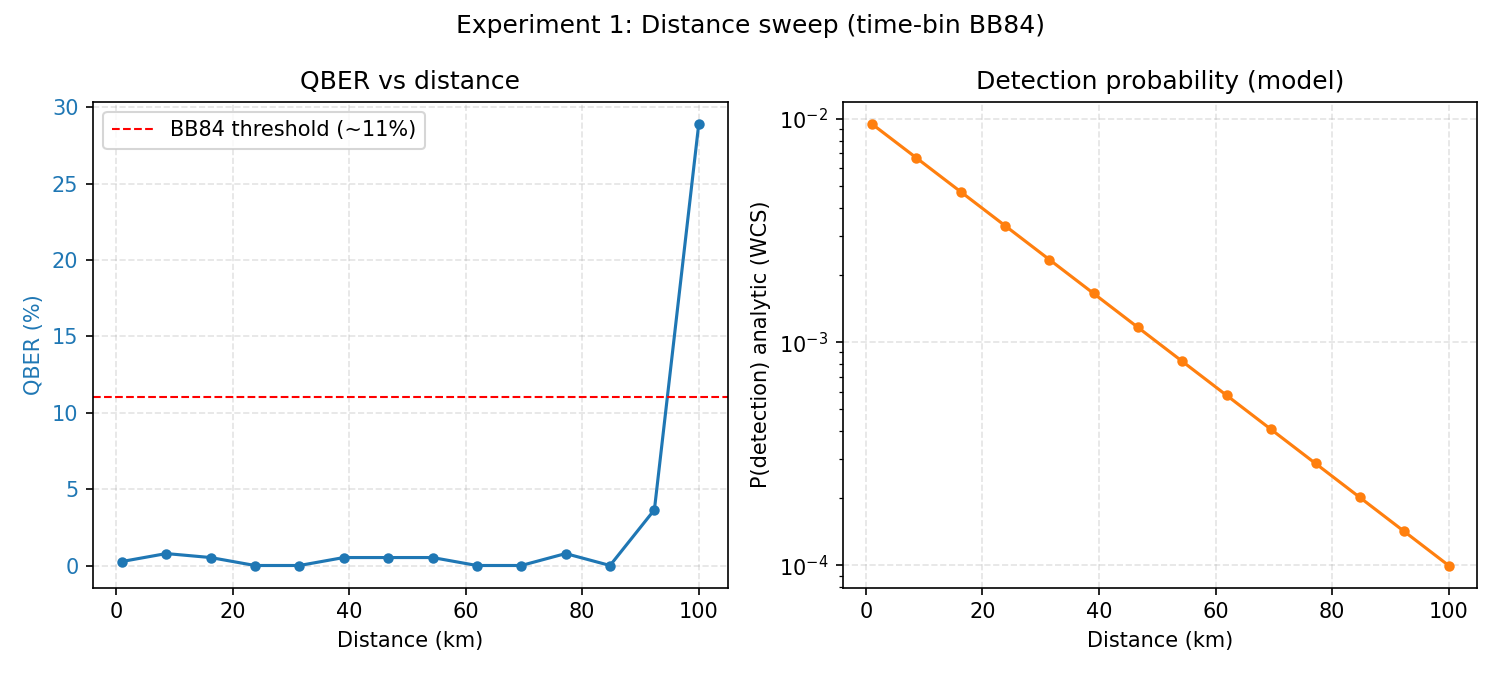
\includegraphics[width=\textwidth]{exp1_distance_sweep.png}
  \caption{QBER y probabilidad de detección en función de la distancia de fibra para BB84 \textit{time-bin}.}
  \label{fig:exp1_distance}
\end{figure}

La Figura~\ref{fig:exp1_skr} presenta la tasa de llave secreta estimada. La tasa cae gradualmente con la distancia mientras el QBER permanece por debajo del umbral, y se anula en la práctica cuando el error excede el margen de seguridad del modelo. La escala logarítmica permite observar tanto la degradación progresiva como la caída final.

\begin{figure}[H]
  \centering
  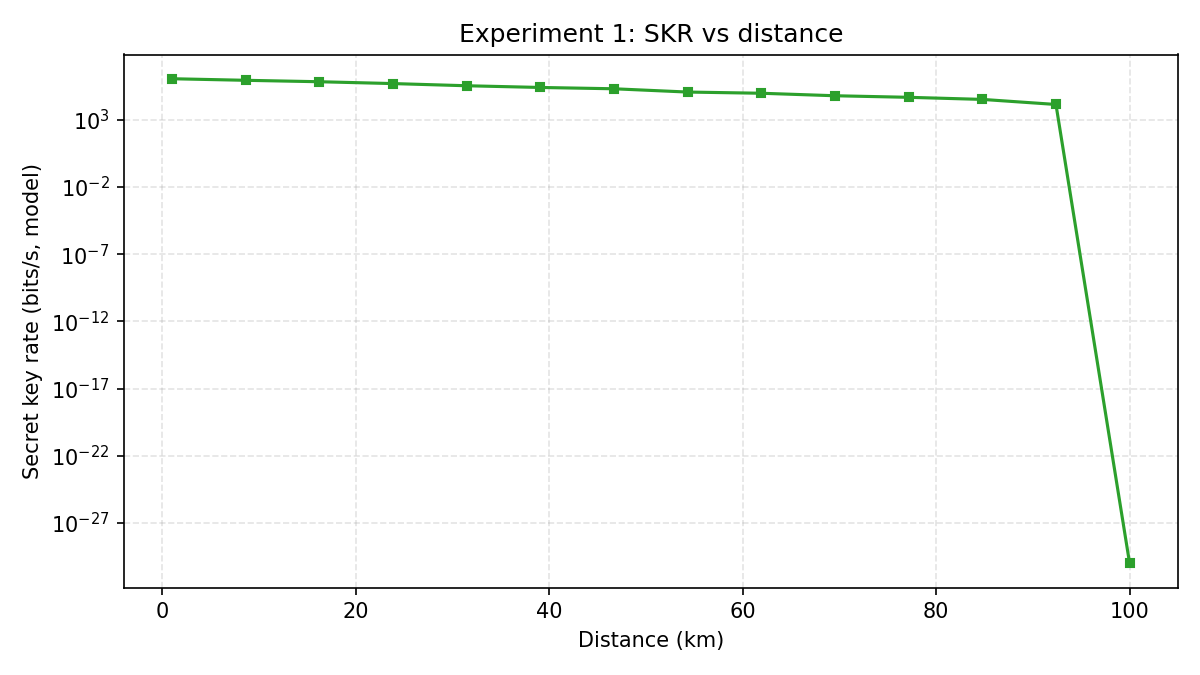
\includegraphics[width=0.92\textwidth]{exp1_skr_distance.png}
  \caption{Tasa de llave secreta estimada en función de la distancia.}
  \label{fig:exp1_skr}
\end{figure}

\section{Sensibilidad del detector}

La Figura~\ref{fig:exp2_detector} resume el impacto de eficiencia y conteos oscuros a \SI{50}{\kilo\meter}. En el barrido de eficiencia, el QBER permanece por debajo del umbral para todos los puntos simulados. La SKR cambia con la eficiencia de detector, aunque el resultado muestra variaciones punto a punto asociadas al carácter estocástico y al tamaño finito de muestra. Esto refuerza que el barrido sirve como indicador de tendencia y sensibilidad, no como predicción determinista punto por punto.

En el barrido de conteos oscuros, el QBER también se mantiene bajo en las condiciones simuladas. La degradación esperada por conteos oscuros no domina fuertemente este conjunto de parámetros, lo que sugiere que, para el banco de pruebas inicial, la eficiencia y la acumulación de eventos válidos pueden ser restricciones más visibles que los conteos oscuros dentro del rango elegido. En una implementación física, este resultado debería revisarse con ventanas temporales, jitter y tasas de repetición reales.

\begin{figure}[H]
  \centering
  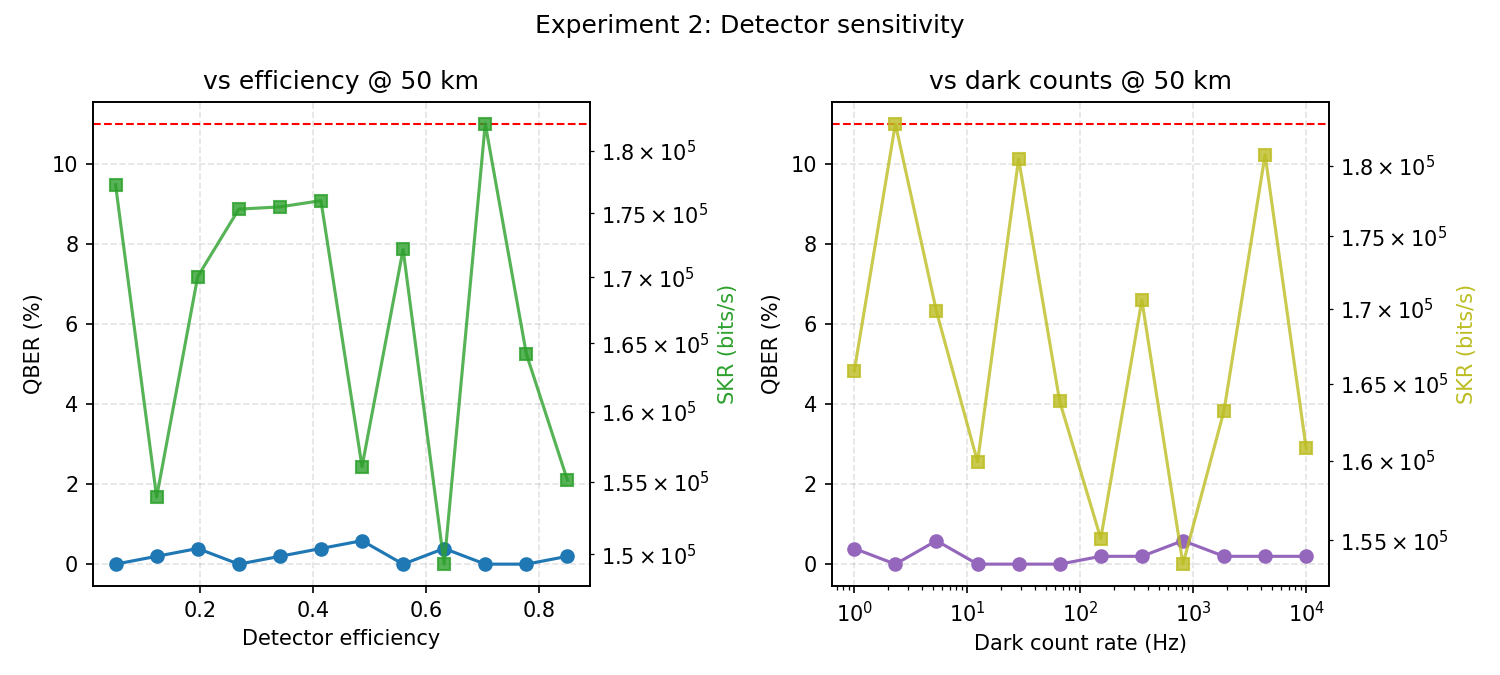
\includegraphics[width=\textwidth]{exp2_detector_sensitivity.png}
  \caption{QBER y SKR frente a eficiencia de detector y conteos oscuros a \SI{50}{\kilo\meter}.}
  \label{fig:exp2_detector}
\end{figure}

\section{Visibilidad interferométrica}

La Figura~\ref{fig:exp3_visibility} muestra el barrido de visibilidad. A medida que la visibilidad mejora, el QBER tiende a disminuir y la SKR se ubica en valores más altos. El efecto no es perfectamente monótono porque la simulación usa llaves cortas y un número limitado de repeticiones; aun así, la relación física principal se conserva: la calidad interferométrica es una variable crítica para una codificación \textit{time-bin}.

Este resultado es importante para el diseño del banco de pruebas. La estabilidad de fase, el balance de caminos ópticos y la resolución temporal del detector no son detalles secundarios, sino condiciones necesarias para que la base de superposición produzca resultados confiables. En consecuencia, el interferómetro y la sincronización deberían considerarse subsistemas de alta prioridad experimental.

\begin{figure}[H]
  \centering
  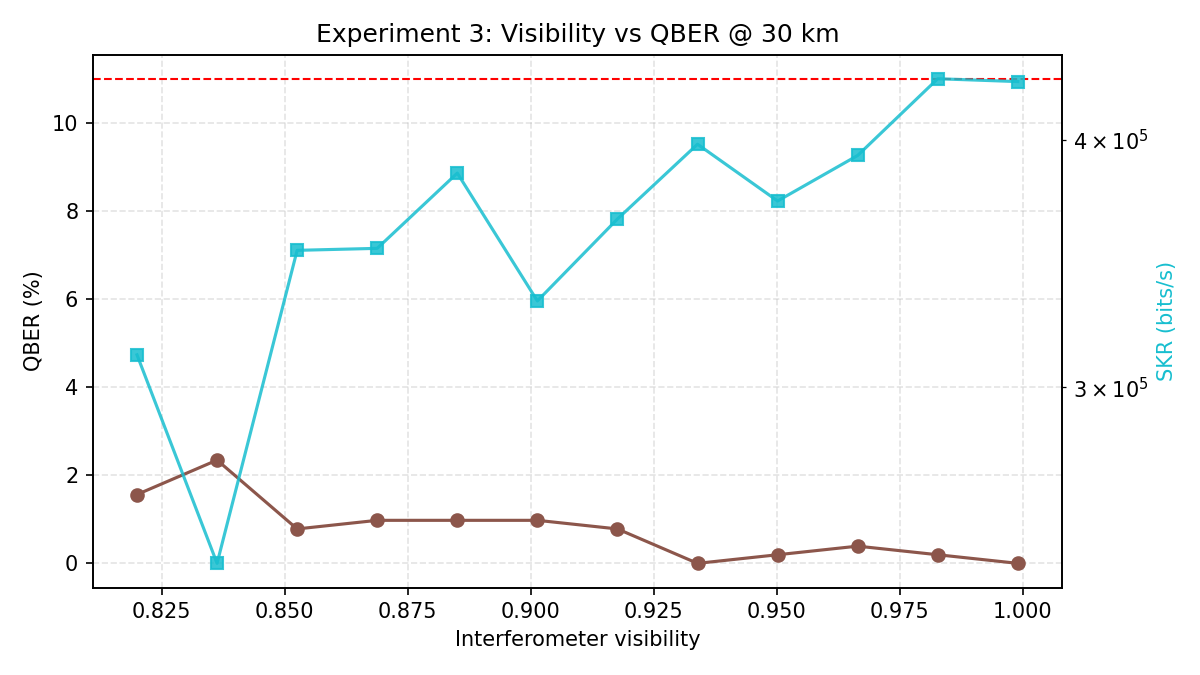
\includegraphics[width=0.92\textwidth]{exp3_visibility.png}
  \caption{QBER y SKR en función de la visibilidad del interferómetro a \SI{30}{\kilo\meter}.}
  \label{fig:exp3_visibility}
\end{figure}

\section{Estados señuelo}

La Figura~\ref{fig:exp4_decoy} compara la estimación sin estados señuelo con la cota analítica decoy. Ambas curvas disminuyen con la distancia. La curva decoy queda por debajo de la estimación simple porque aplica una cota más conservadora sobre la contribución segura de eventos monofotónicos. Por lo tanto, el resultado no implica que los estados señuelo empeoren el sistema; indica que la tasa segura certificable bajo ese modelo es menor que una estimación simple que no contempla la misma exposición a pulsos multifotónicos.

Para un banco de pruebas real, la lectura correcta es que los estados señuelo agregan complejidad experimental y de procesamiento, pero son relevantes para acercar la estimación de tasa a un modelo de seguridad más realista con fuentes coherentes débiles. El paso siguiente sería implementar selección aleatoria de intensidades y estimación estadística dentro del flujo protocolar, en lugar de calcular la cota como postproceso analítico.

\begin{figure}[H]
  \centering
  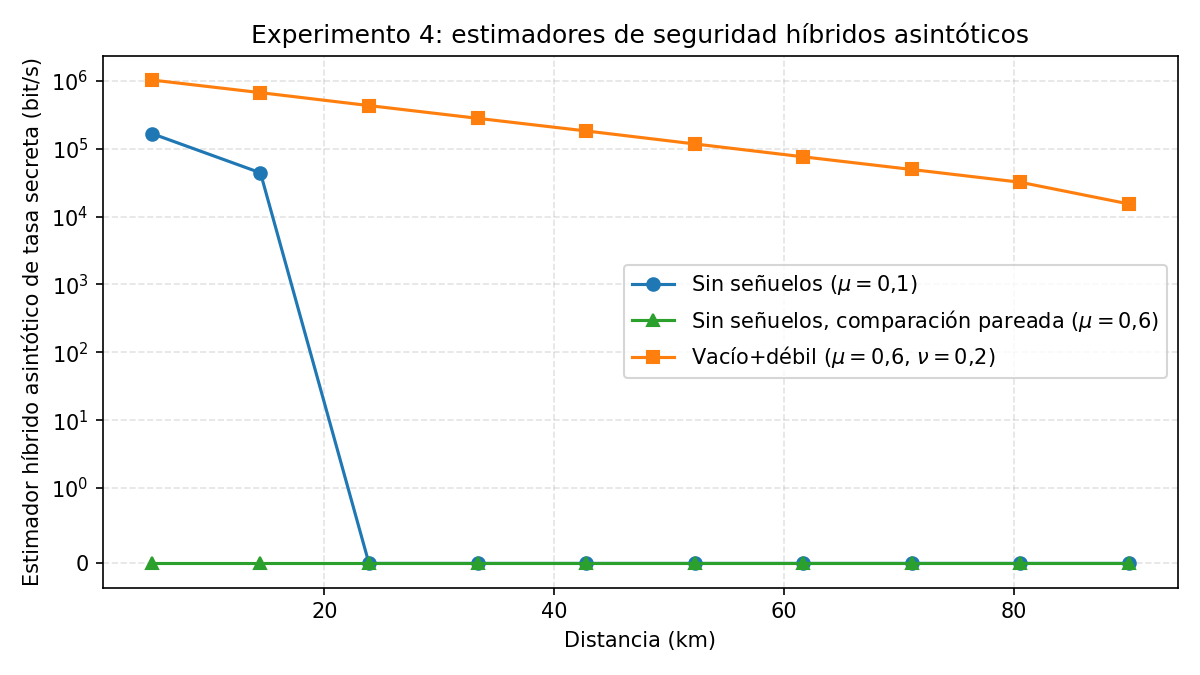
\includegraphics[width=0.92\textwidth]{exp4_decoy_impact.png}
  \caption{Comparación de SKR modelo sin estados señuelo y cota analítica con estados señuelo.}
  \label{fig:exp4_decoy}
\end{figure}

\section{Síntesis de resultados}

\begin{table}[H]
  \centering
  \begin{tabular}{p{0.25\textwidth}p{0.64\textwidth}}
    \toprule
    Barrido & Conclusión de diseño \\
    \midrule
    Distancia & La atenuación reduce la probabilidad de detección y termina anulando la SKR cuando el QBER supera el umbral. \\
    Detector & La eficiencia afecta la tasa útil; los conteos oscuros del rango probado no dominan el error bajo estos parámetros. \\
    Visibilidad & La calidad interferométrica es crítica para \textit{time-bin}; visibilidad baja aumenta QBER y reduce SKR. \\
    Estados señuelo & La cota decoy es más conservadora y representa mejor el riesgo de pulsos multifotónicos en fuentes coherentes débiles. \\
    \bottomrule
  \end{tabular}
  \caption{Resumen de conclusiones experimentales para el diseño del banco de pruebas.}
  \label{tab:sintesis_resultados}
\end{table}

\chapter{Conclusiones}
\label{chap:conclusiones}

\section{Respuesta a la hipótesis}

La hipótesis se sostiene dentro del alcance definido: una simulación de eventos discretos permite convertir el diseño de un banco QKD en preguntas medibles, cuantificar la variación entre corridas y detectar cuándo una salida exige revisar sus supuestos. El trabajo no confirma la factibilidad física del Campus Miguelete ni certifica seguridad criptográfica.

Los cuatro criterios de verificación se cumplen. La evidencia conserva parámetros, semillas, bits, errores, tiempos y clics; cada punto contiene \PThreeRepetitions{} repeticiones; el flujo comprueba invariantes numéricos; y la referencia analítica detecta una pérdida de holgura que la lectura aislada de QBER no habría mostrado. Este último resultado es importante: la utilidad de la simulación no consiste sólo en producir curvas plausibles, sino también en impedir que una tasa incoherente se transforme en especificación de diseño.

\section{Cumplimiento de objetivos}

\begin{table}[htbp]
  \centering
  \small
  \begin{tabularx}{\textwidth}{p{0.27\textwidth}p{0.18\textwidth}X}
    \toprule
    Objetivo & Estado & Evidencia \\
    \midrule
    Escenario Alice--Bob \textit{time-bin} & Cumplido & SeQUeNCe 0.8.5, componentes, canales y parche identificados \\
    Barrido de distancia & Cumplido con límite & Transición de control entre \num[round-mode=places,round-precision=2]{\PThreeTransitionLowKm} y \SI[round-mode=places,round-precision=2]{\PThreeTransitionHighKm}{\kilo\meter}; no es alcance físico \\
    Sensibilidad del detector & Cumplido, no concluyente & Los IC de eficiencia y fondo incluyen cero \\
    Sensibilidad a visibilidad & Cumplido internamente & Pendiente QBER negativa, con doce puntos sin holgura de tasa \\
    Comparación señuelo & Cumplido como estimador & Igual \(\mu\), cota asintótica híbrida y reemplazos conservadores registrados \\
    Diseño Campus Miguelete & Parcial & Topología y criterios definidos; faltan ruta y pérdidas medidas \\
    Trazabilidad & Cumplido & 60 agregados, 1.800 registros, 2.100 ejecuciones, macros y hashes \\
    \bottomrule
  \end{tabularx}
  \caption{Respuesta de la evidencia a los objetivos del trabajo.}
  \label{tab:objetivos_cierre}
\end{table}

\section{Conclusiones por experimento}

El barrido de distancia reproduce la caída de ganancia, pero su conclusión principal no es una distancia máxima. Entre \num[round-mode=places,round-precision=2]{\PThreeTransitionLowKm} y \SI[round-mode=places,round-precision=2]{\PThreeTransitionHighKm}{\kilo\meter}, la tasa tamizada deja de conservar holgura frente a la referencia. Los puntos posteriores sirven para auditar temporización y detecciones, no para defender prestaciones.

El experimento de detector no resuelve los efectos entre extremos. Para eficiencia, el intervalo de \(\Delta I\) va de \num[round-mode=places,round-precision=1]{\PThreeEffDifferenceLowKbps} a \num[round-mode=places,round-precision=1]{\PThreeEffDifferenceHighKbps}\,kbit/s y \(p=\num[round-mode=places,round-precision=3]{\PThreeEffPValue}\). Para fondo, va de \num[round-mode=places,round-precision=1]{\PThreeDarkDifferenceLowKbps} a \num[round-mode=places,round-precision=1]{\PThreeDarkDifferenceHighKbps}\,kbit/s y \(p=\num[round-mode=places,round-precision=3]{\PThreeDarkPValue}\). Esto impide ordenar detectores a partir de estas curvas. Una comparación de hardware debe incorporar ventanas, tiempo muerto, fluctuación temporal y pérdidas internas medidas.

El barrido de visibilidad confirma una pendiente negativa de QBER. Era esperable porque \(p_\mathrm{fase}\) se calcula desde \(V\); el resultado demuestra que la dependencia llega a BB84 después de corregir el interferómetro. No demuestra estabilidad física. Los doce puntos carecen de holgura de tasa, de modo que el valor absoluto del indicador no se usa como evidencia de factibilidad.

La comparación de estados señuelo muestra la utilidad de estimar la contribución monofotónica. Con igual \(\mu=0{,}1\), la tasa sin señuelos se anula cerca de \SI{24}{\kilo\meter}, mientras la estimación señuelo conserva \SI[round-mode=places,round-precision=1]{\PThreeDecoyTwentyFourKbps}{\kilo bit\per\second}. El resultado depende de ganancias analíticas, error de fase aproximado y tratamiento asintótico. Los \PThreeDecoyFallbackTotal{} reemplazos conservadores en 300 repeticiones pareadas deben considerarse al interpretar la media.

\section{Aporte para la implementación UNSAM}

El trabajo entrega una secuencia concreta para la siguiente etapa. Primero se mide una ruta óptica y se registra cada pérdida fija. Después se selecciona una combinación coherente de fuente, moduladores, detector, registro temporal e interferómetro. Esos valores restringen el dominio del simulador. Finalmente, se compara una medición corta con la salida del modelo y se ajustan temporización, fondo y visibilidad.

El presupuesto y las imágenes de equipos cumplen una función de preselección, no de compra. Los rangos de costo son orientativos y no provienen de cotizaciones vigentes. Antes de adquirir equipos se necesita una tabla con cantidad, modelo exacto, accesorios, precio, fecha, importación y contingencia. Sin ese paso, sumar mínimos y máximos produce un número aparente pero no un presupuesto ejecutable.

\section{Limitaciones}

Las principales limitaciones son:

\begin{itemize}
  \item la referencia de tasa no reproduce toda la temporización interna y detecta una discrepancia todavía no resuelta;
  \item la ventana de \SI{1}{\nano\second} es analítica y no una compuerta implementada en el receptor;
  \item el barrido de eficiencia excede la especificación del detector comercial usado como referencia;
  \item el modelo no separa errores por base ni ejecuta autenticación, reconciliación y amplificación de privacidad;
  \item el estimador señuelo es asintótico, híbrido y no componible;
  \item no se modelan ataques laterales, deriva térmica, dispersión, pérdidas internas ni calibración dinámica;
  \item el campus no cuenta aún con una ruta óptica medida ni una lista de materiales cotizada.
\end{itemize}

\section{Trabajo futuro priorizado}

La primera prioridad es resolver la diferencia entre tasa tamizada y referencia. Para ello debe instrumentarse el tiempo efectivo de emisión, la cantidad de pulsos, los clics aceptados y el instante usado en el denominador. La prueba debe cubrir el intervalo de \num[round-mode=places,round-precision=2]{\PThreeTransitionLowKm} a \SI[round-mode=places,round-precision=2]{\PThreeTransitionHighKm}{\kilo\meter} y el escenario de visibilidad.

La segunda prioridad es medir una ruta del Campus Miguelete con OTDR o instrumentación equivalente. El resultado debe incluir longitud óptica, atenuación total, conectores, empalmes, fibras disponibles y restricciones de acceso. Con esos datos puede calcularse un presupuesto de enlace específico.

La tercera prioridad es definir una configuración de laboratorio coherente. Deben elegirse modelos exactos de fuente, moduladores, detector y registrador temporal; después se reemplazan los barridos amplios por rangos compatibles con sus hojas de datos y cotizaciones.

La cuarta prioridad es avanzar desde estimadores a protocolo. Esto requiere elegir intensidades dentro de la ejecución, separar estadísticas por base e intensidad, implementar reconciliación, verificación, amplificación de privacidad y autenticación, y aplicar análisis de clave finita.

\section{Cierre}

El trabajo no demuestra que UNSAM pueda desplegar hoy un enlace QKD operativo. Demuestra algo anterior y necesario: cómo construir una simulación auditable, cómo distinguir métricas de desempeño de tasas con interpretación criptográfica y cómo detectar límites antes de comprar hardware. Esa base permite que la siguiente decisión se apoye en datos medidos y no en una extrapolación de curvas.


\appendix
\chapter{Reproducción del experimento}
\label{app:reproduccion}

\section{Fuentes autoritativas}

\begin{itemize}
  \item \texttt{experiments/proyecto3\_simulation.py}: flujo estadístico que genera la evidencia de la tesis.
  \item \texttt{experiments/results/}: CSV agregados, CSV por repetición, figuras, macros y manifiesto.
  \item \texttt{sequence/qkd/BB84.py}: implementación BB84 usada por \texttt{QKDNode}.
  \item \texttt{sequence/topology/node.py}: nodos y receptor \textit{time-bin}.
  \item \texttt{sequence/components/detector.py}: clases base y detector \textit{time-bin}.
  \item \texttt{sequence/components/interferometer.py}: interferómetro con la corrección local de \texttt{phase\_error}.
  \item \texttt{paper/main.tex}: documento completo.
\end{itemize}

El archivo \texttt{experiments/qkd\_2node\_simulation.py} es un lanzador de demostraciones separadas. No debe usarse para reconstruir las figuras de esta versión porque no genera el mismo diseño estadístico.

\section{Entorno}

El repositorio fija dependencias en \texttt{pyproject.toml} y \texttt{uv.lock}. Desde la raíz:

\begin{verbatim}
uv sync
\end{verbatim}

El manifiesto de resultados registra hashes de ambos archivos de dependencias, del flujo, de BB84 y de los módulos de nodo, detector e interferómetro. La versión efectiva del simulador es SeQUeNCe 0.8.5 más las correcciones locales documentadas.

\section{Generación de datos y figuras}

\begin{verbatim}
uv run python experiments/proyecto3_simulation.py \
  --repetitions 30 --workers 8
\end{verbatim}

El número de trabajadores sólo modifica el paralelismo. Cada corrida recibe semillas deterministas antes de distribuirse entre procesos, por lo que la evidencia no depende del orden de finalización. La ejecución genera:

\begin{itemize}
  \item \texttt{exp1\_distance\_data.csv} y \texttt{exp1\_distance\_runs.csv};
  \item \texttt{exp2\_detector\_data.csv} y \texttt{exp2\_detector\_runs.csv};
  \item \texttt{exp3\_visibility\_data.csv} y \texttt{exp3\_visibility\_runs.csv};
  \item \texttt{exp4\_decoy\_data.csv} y \texttt{exp4\_decoy\_runs.csv};
  \item cinco figuras PNG;
  \item \texttt{proyecto3\_results.tex}, con las macros numéricas;
  \item \texttt{experiment\_summary.json}, con métodos, parámetros, filas y hashes.
\end{itemize}

Los cuatro CSV agregados contienen 60 filas y los archivos detallados contienen 1.800 registros de repetición. En el experimento señuelo, cada registro combina dos ejecuciones; el total real es de 2.100 ejecuciones de SeQUeNCe. El flujo se detiene si falla un invariante numérico o si los parámetros efectivos de un detector difieren de la configuración solicitada. El número de claves completadas se exporta y los datos actuales cumplen lo solicitado, pero esa igualdad todavía no se fuerza mediante una aserción.

\section{Compilación del documento}

Desde la carpeta \texttt{paper/}:

\begin{verbatim}
tectonic --keep-logs main.tex
\end{verbatim}

La compilación importa \texttt{../experiments/results/proyecto3\_results.tex}. De este modo, los valores principales del resumen, resultados y conclusiones provienen de la ejecución. Tectonic no vuelve a correr el simulador; generación y composición son pasos separados.

\section{Trazabilidad de figuras}

\begin{table}[htbp]
  \centering
  \footnotesize
  \begin{tabularx}{\textwidth}{>{\raggedright\arraybackslash}p{0.16\textwidth}>{\raggedright\arraybackslash}p{0.36\textwidth}>{\raggedright\arraybackslash}X}
    \toprule
    Figura & Función de experimento & Archivo \\
    \midrule
    QBER & \path{experiment_1_distance_sweep} & \path{exp1_distance_sweep.png} \\
    Indicador ideal & \path{experiment_1_distance_sweep} & \path{exp1_skr_distance.png} \\
    Detector & \path{experiment_2_detector_sweep} & \path{exp2_detector_sensitivity.png} \\
    Visibilidad & \path{experiment_3_visibility_sweep} & \path{exp3_visibility.png} \\
    Señuelos & \path{experiment_4_decoy_distance} & \path{exp4_decoy_impact.png} \\
    \bottomrule
  \end{tabularx}
  \caption{Correspondencia entre funciones y figuras del trabajo.}
  \label{tab:trazabilidad_figuras}
\end{table}

\section{Verificación independiente}

Para revisar una cifra sin repetir el experimento se parte del CSV de repeticiones. QBER se recalcula sumando errores y bits; las tasas se recalculan con las 30 observaciones de cada punto. Después se comparan los resultados con el CSV agregado y con las macros LaTeX. Los hashes del manifiesto comprueban la identidad del código, las dependencias, los CSV y las macros. No incluyen las figuras, las fuentes LaTeX ni el PDF; la correspondencia documental se verifica compilando las fuentes versionadas que importan esas macros. Una identidad exacta del PDF requiere además conservar el archivo compilado o su hash en el mismo commit.

La reproducibilidad computacional no elimina la dependencia del entorno. Diferencias de arquitectura, bibliotecas numéricas o versión de SeQUeNCe pueden cambiar detalles de punto flotante. Por eso el manifiesto conserva versiones y hashes, y los resultados se interpretan mediante intervalos y no por igualdad exacta de todos los decimales.

\chapter{Fragmentos de código relevantes}
\label{app:codigo}

Este apéndice selecciona principalmente fragmentos de \path{experiments/proyecto3_simulation.py}. El ejemplo de bootstrap reproduce un control post hoc aplicado a los CSV y se identifica como tal; no pertenece al generador autoritativo. El objetivo es mostrar cómo las decisiones metodológicas se traducen a código. Los recortes no reemplazan los archivos ejecutables ni sus validaciones.

\section{Parámetros y semillas}

\begin{lstlisting}[language=Python, caption={Contrato de parámetros de una corrida.}]
@dataclass
class SimParams:
    distance_km: float
    attenuation_db_km: float = DEFAULT_ALPHA_DB_KM
    detector_efficiency: float = 0.1
    dark_count_hz: float = 100.0
    mean_photon_num: float = 0.1
    frequency_hz: float = DEFAULT_FREQUENCY_HZ
    visibility: float = 0.98
    key_length: int = DEFAULT_KEY_LENGTH
    num_keys: int = DEFAULT_NUM_KEYS
    runtime_ps: float = DEFAULT_RUNTIME_PS
    alice_seed: int = 0
    bob_seed: int = 1
    count_rate_hz: float = 50e6
    time_resolution_ps: int = 10
    detection_window_ps: int = DEFAULT_DETECTION_WINDOW_PS
    classical_extra_delay_ps: int = DEFAULT_CLASSICAL_EXTRA_DELAY_PS
\end{lstlisting}

\texttt{SimParams} separa la configuración del motor de simulación. Cada barrido crea una instancia y modifica sólo los campos definidos por su diseño. La ventana de detección aparece en la misma estructura, pero se usa en la referencia analítica de fondo; no configura una compuerta física de SeQUeNCe. Esta diferencia evita atribuir al receptor una función que no implementa.

\begin{lstlisting}[language=Python, caption={Semilla común para las fuentes aleatorias del modelo.}]
def _seed_simulation(alice_seed: int, bob_seed: int) -> int:
    simulation_seed = (
        (alice_seed * 1_000_003) ^ bob_seed
    ) & 0xFFFFFFFF
    np.random.seed(simulation_seed)
    random.seed(simulation_seed)
    Timeline.seed(simulation_seed)
    return simulation_seed
\end{lstlisting}

La corrida usa varias fuentes de aleatoriedad. Sembrar sólo NumPy no alcanza: también se fijan el módulo estándar y la línea temporal. Alice y Bob reciben, además, sus semillas de nodo. El flujo asigna pares no superpuestos por punto y repetición. Así puede reconstruirse una observación sin hacer idénticas todas las corridas.

\section{Enlace y parche de visibilidad}

\begin{lstlisting}[language=Python, caption={Creación abreviada del enlace y configuración del receptor.}]
tl = Timeline(p.runtime_ps)
qc0 = QuantumChannel(
    "qc0", tl, distance=distance_m,
    attenuation=attenuation_db_m,
    frequency=p.frequency_hz,
)
cc0 = ClassicalChannel("cc0", tl, distance=distance_m)
cc0.delay += p.classical_extra_delay_ps

alice = QKDNode("alice", tl, encoding=time_bin, stack_size=1)
bob = QKDNode("bob", tl, encoding=time_bin, stack_size=1)

phase_error = max(0.0, min(1.0, (1.0 - p.visibility) / 2.0))
qsd = bob.components["bob.qsdetector"]
qsd.update_interferometer_params("phase_error", phase_error)
\end{lstlisting}

La distancia y atenuación se aplican al canal cuántico, mientras el retardo adicional pertenece al canal clásico. El experimento de detector fija este último en cero para reducir su influencia sobre la tasa. La visibilidad se transforma en error de fase y llega al interferómetro.

La versión base de SeQUeNCe 0.8.5 no aplicaba correctamente ese error a \texttt{FreeQuantumState}. El repositorio corrige \path{sequence/components/interferometer.py}. Sin el parche, barrer \(V\) no produciría la respuesta documentada; por eso su hash forma parte del manifiesto.

\section{Tasa agregada y referencia}

\begin{lstlisting}[language=Python, caption={Cálculo de la tasa tamizada de una repetición.}]
bb_a = alice.protocol_stack[0]
errs = list(getattr(bb_a, "error_rates", []) or [])
n_keys = len(errs)
total_sifted_bits = n_keys * p.key_length
total_errors = int(round(sum(errs) * p.key_length))
mean_qber = (
    total_errors / total_sifted_bits
    if total_sifted_bits else float("nan")
)

elapsed_key_ps = float(getattr(bb_a, "last_key_time", 0.0))
elapsed_key_s = elapsed_key_ps * 1e-12
aggregate_throughput = (
    total_sifted_bits / elapsed_key_s
    if elapsed_key_s > 0 else 0.0
)
\end{lstlisting}

SeQUeNCe expone una tasa de error por clave completada en \texttt{error\_rates}; no expone aquí las claves tamizadas como atributos públicos. El script reconstruye el conteo total de errores multiplicando la suma de esas tasas por la longitud de clave y redondeando al entero más cercano. Luego calcula QBER con los conteos agregados, no promediando porcentajes por clave. La tasa divide todos los bits tamizados por el tiempo simulado hasta la última clave. Promediar tasas instantáneas asignaría el mismo peso a intervalos de distinta duración y podría sesgar la salida.

\begin{lstlisting}[language=Python, caption={Fondo, ganancia y referencia de clics tamizados.}]
def background_yield(dark_count_hz, detection_window_ps,
                     detectors=3):
    exposure_s = detectors * detection_window_ps * 1e-12
    return 1.0 - math.exp(-dark_count_hz * exposure_s)

def wcs_gain(mu, eta_channel, eta_det, y0):
    no_signal_click = math.exp(-mu * eta_channel * eta_det)
    return 1.0 - (1.0 - y0) * no_signal_click

y0 = background_yield(p.dark_count_hz, p.detection_window_ps)
q_mu = wcs_gain(p.mean_photon_num, eta_ch,
                p.detector_efficiency, y0)
sifted_rate_reference = 0.5 * min(
    p.frequency_hz * q_mu,
    3 * p.count_rate_hz,
)
\end{lstlisting}

\texttt{background\_yield} convierte tasa oscura y ventana supuesta en probabilidad por pulso para tres detectores. \texttt{wcs\_gain} combina ese fondo con la probabilidad de no recibir señal. El factor \(1/2\) representa tamizado por bases y el mínimo impone disponibilidad de pulsos o límite agregado de conteo. La referencia es un control medio; no se programa como tope de cada corrida.

\section{Indicador ideal}

\begin{lstlisting}[language=Python, caption={Indicador de posprocesamiento monofotónico ideal.}]
def ideal_postprocessing_rate(qber, r_sifted_bps,
                              f_ec=1.16):
    if (not math.isfinite(qber)
            or qber < 0 or qber >= 0.5):
        return 0.0
    h = _binary_entropy(qber)
    factor = max(0.0, 1.0 - f_ec * h - h)
    return r_sifted_bps * factor
\end{lstlisting}

La función no fija un corte manual en 11\%. El factor se anula por su propia entropía cerca de 9,81\% cuando \(f_\mathrm{EC}=1{,}16\). Su nombre evita una afirmación que el cálculo no sostiene: para una fuente coherente débil sin estimación monofotónica, el resultado no es una tasa secreta.

\section{Intervalos y contrastes}

\begin{lstlisting}[language=Python, caption={Intervalo de Wilson para QBER agrupada.}]
def _wilson_qber_ci(runs, confidence=0.95):
    errors = sum(run["total_errors"] for run in runs)
    bits = sum(run["total_sifted_bits"] for run in runs)
    p = errors / bits
    z = stats.norm.ppf((1.0 + confidence) / 2.0)
    denom = 1.0 + z * z / bits
    center = (p + z * z / (2.0 * bits)) / denom
    half = (
        z * math.sqrt(
            p * (1.0 - p) / bits
            + z * z / (4.0 * bits * bits)
        ) / denom
    )
    return p, max(0.0, center-half), min(1.0, center+half)
\end{lstlisting}

QBER es una proporción y puede estar cerca de cero. Wilson conserva mejor comportamiento que la aproximación normal simple en ese régimen, siempre que los bits agrupados puedan tratarse como intercambiables. No captura dependencia dentro de una clave ni heterogeneidad entre repeticiones. Las tasas usan intervalos t porque cada repetición produce una observación continua; las diferencias de detector usan Welch para no imponer varianzas iguales.

Como control posterior, las medias señuelo se remuestrean a nivel de repetición:

\begin{lstlisting}[language=Python, caption={Bootstrap percentil usado como análisis de sensibilidad.}]
rng = np.random.default_rng(20260901)
indices = rng.integers(
    0, rates.size, size=(100_000, rates.size)
)
bootstrap_means = rates[indices].mean(axis=1)
ci_bootstrap = np.quantile(
    bootstrap_means, [0.025, 0.975]
)
\end{lstlisting}

Este cálculo usa las 30 tasas ya exportadas y no vuelve a ejecutar SeQUeNCe. El remuestreo conserva como unidad la repetición completa, por lo que tolera asimetría y valores nulos mejor que una justificación puramente normal \cite{efron1979bootstrap}. Para visibilidad se usa además HC3, que pondera cada residuo por \((1-h_{ii})^{-2}\) y reduce la dependencia del intervalo respecto de homoscedasticidad \cite{mackinnonWhite1985}. Ninguno de estos controles convierte los resultados en cotas de clave finita.

\section{Cota señuelo y caso conservador}

\begin{lstlisting}[language=Python, caption={Cota de error monofotónico con reemplazo conservador.}]
def decoy_e1_upper(e_nu, q_nu, e0, y0, y1, nu):
    if y1 <= 0 or nu <= 0:
        return 0.5
    numerator = e_nu * q_nu * math.exp(nu) - e0 * y0
    if numerator <= 0:
        return 0.5
    return min(0.5, numerator / (y1 * nu))
\end{lstlisting}

Un numerador no positivo aparece cuando la combinación de error simulado, ganancia analítica y muestra finita no sostiene una cota positiva. Truncarlo a cero supondría ausencia de error y aumentaría la tasa. El código adopta \(1/2\), que anula la contribución secreta de esos eventos. El flujo cuenta cada activación para que la media no oculte esta decisión.

\section{Validaciones y manifiesto}

\begin{lstlisting}[language=Python, caption={Ejemplos de invariantes verificados antes de exportar.}]
assert 0.0 <= qber <= 0.5
assert qber_low <= qber <= qber_high
assert 0.0 <= ideal_rate <= sifted_rate
assert 0.0 <= q_nu <= q_mu <= 1.0
assert detector_sum == total_detector_clicks
for detector in qsd.detectors:
    for name, expected in effective_detector_params.items():
        if getattr(detector, name) != expected:
            raise RuntimeError(f"{name} was not applied")
\end{lstlisting}

Las aserciones detienen la generación si una salida viola las definiciones implementadas. No comprueban todavía que cada ejecución complete exactamente el número de claves solicitado. Después, el script calcula SHA-256 del flujo, el parche, las dependencias, cada CSV y las macros numéricas. Los hashes no prueban corrección científica ni cubren las fuentes LaTeX, las figuras o el PDF; prueban identidad de la evidencia computacional registrada.


\bibliographystyle{ieeetr}
\bibliography{references}

\end{document}
